\documentclass[t]{beamer}
\usetheme{Copenhagen}
\setbeamertemplate{headline}{} % remove toc from headers
\beamertemplatenavigationsymbolsempty

\usepackage{amsmath, array, tikz, bm, pgfplots, tcolorbox, graphicx, venndiagram, color, colortbl, xfrac}
\pgfplotsset{compat = 1.16}
\usepgfplotslibrary{statistics}
\usetikzlibrary{calc}

\title{Sampling Distributions}
\author{}
\date{}

\AtBeginSection[]
{
  \begin{frame}
    \frametitle{Objectives}
    \tableofcontents[currentsection]
  \end{frame}
}

\begin{document}

\begin{frame} 
\maketitle
\end{frame}

\section{Obtain a sampling distribution of sample means}

\begin{frame}{Sampling Distributions}
In statistics, we take samples in order to gather information regarding a population. \newline\\	\pause

For instance, let's say we have the following population prices of laptops: \$1000, \$1200, \$1600, and \$2000.	\newline\\	\pause

We can take a simple random sample of, say 2 computers, and create a frequency distribution of each sample.	\newline\\	\pause

\emph{Note}: We will sample with replacement. Differences in sampling with and without replacement become negligent as sample sizes increase.
\end{frame}

\begin{frame}{Example 1}
Obtain a sampling distribution, taking 2 at a time, of the laptop prices \$1000, \$1200, \$1600, and \$2000. Then find the mean of each sample.	\newline\\	\pause
\begin{minipage}{0.4\textwidth}
\begin{tabular}{c|c}
Sample & Sample Mean \\ \hline
1000, 1000 & 1000 \\
1000, 1200 & 1100 \\
1000, 1600 & 1300 \\
1000, 2000 & 1500 \\
1200, 1000 & 1100 \\
1200, 1200 & 1200 \\
1200, 1600 & 1400 \\
1200, 2000 & 1600 \\
\end{tabular}
\end{minipage}
\hspace{0.5cm}
\begin{minipage}{0.4\textwidth}
\begin{tabular}{c|c}
Sample & Sample Mean \\ \hline
1600, 1000 & 1300 \\
1600, 1200 & 1400 \\
1600, 1600 & 1600 \\
1600, 2000 & 1800 \\
2000, 1000 & 1500 \\
2000, 1200 & 1600 \\
2000, 1600 & 1800 \\
2000, 2000 & 2000 \\
\end{tabular}
\end{minipage}
\end{frame}

\begin{frame}{Example 2}
Create a histogram of the sample means from Example 1.	\newline\\	\pause
\begin{center}
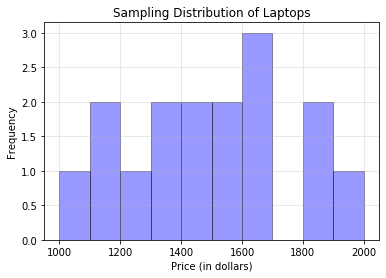
\includegraphics[scale=0.6]{../Images/sampling_hist_01.png}
\end{center}
\end{frame}

\begin{frame}{Example 3}
Determine the mean and standard deviation of the sample means.	\newline\\	\pause

$\text{Mean} = \$1450$ \newline\\	\pause

$\text{Std. Dev} \approx \$271.57$
\end{frame}

\section{Determine the mean and standard error of a sampling distribution}

\begin{frame}{Larger Population and Sample Sizes}
What happens if we have a much larger population and take a larger sample size, such as 100?	\newline\\	\pause

Notice that the mean of the sample means targets the population mean. 	\pause

\[\mu \approx \mu_{\overline{x}}\]		\pause

Also, the standard deviation is around 1/10 the population standard deviation. 	\pause

\[\sigma \approx \frac{\sigma_{\overline{x}}}{\sqrt{n}}\]

where $\frac{\sigma}{\sqrt{n}}$ is called the {\color{blue}\textbf{standard error of the mean}}.
\end{frame}

\begin{frame}{Example 4}
IQ scores are normally distributed with a mean of 100 and standard deviation of 16. A sample of 200 participants had their IQs measured.	\pause
\begin{center}
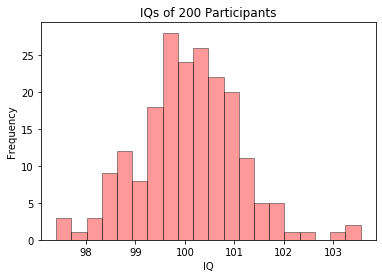
\includegraphics[scale=0.45]{../Images/sample_means_IQ.png}
\end{center}
\smallskip	\pause
What are the approximate mean and standard error of the sample?
\end{frame}

\begin{frame}{Example 4}
The mean of the sample will target the population mean of 100. \newline\\	\pause

The standard error is 
\begin{align*}
\onslide<3->{\frac{\sigma}{\sqrt{n}} &= \frac{16}{\sqrt{200}}} \\[8pt]
\onslide<4->{& \approx 1.13}
\end{align*}
\end{frame}

\section{Understand the Central Limit Theorem}

\begin{frame}{Sample Means of Any Distribution}
We can create a histogram of a population, but how will our histograms of sample means look for various populations?	\newline\\	\pause

It turns out that the distributions of sample means for \underline{any} population will be normal as our sample sizes increase.
\end{frame}

\begin{frame}{Central Limit Theorem}
\begin{center}
{\color{blue}\textbf{\Large Central Limit Theorem}}
\end{center}
As the sample size increases, the distribution of sample means becomes normal with a mean of $\overline{x}$ and standard deviation $\frac{\sigma}{\sqrt{n}}$ (the standard error).
\end{frame}
% Central Limit Theorem

\section{Determine the mean and standard error for sampling distribution of proportions}

\section{Determine the mean and standard error for sampling distribution of variances}
% Sampling distribution of proportions
% Sampling distribution of variances

\end{document}